\documentclass[11pt]{article}
\usepackage[letterpaper,landscape,margin=0.55in]{geometry}
\usepackage{graphicx,booktabs,amsmath,array,fancyhdr,xcolor}
\usepackage[T1]{fontenc}
\usepackage{lmodern}
\setlength{\parindent}{0pt}
\setlength{\parskip}{5pt}
\pagestyle{fancy}\fancyhf{}\fancyfoot[C]{\thepage}
\renewcommand{\headrulewidth}{0pt}
\newcommand{\titleline}[1]{{\Large\bfseries #1}\par\vspace{3pt}}
\begin{document}
\titleline{Theory benchmark: optimized prices}
\small
Normal gamma: mean 0, SD 1.25; $\beta=2$, $\alpha=-1$, zero marginal cost, $\delta=1$.
Uniform observes history but not gamma; Informed observes its quintile. Neither learns.
All offered prices are constrained to be nonnegative.
\begin{center}
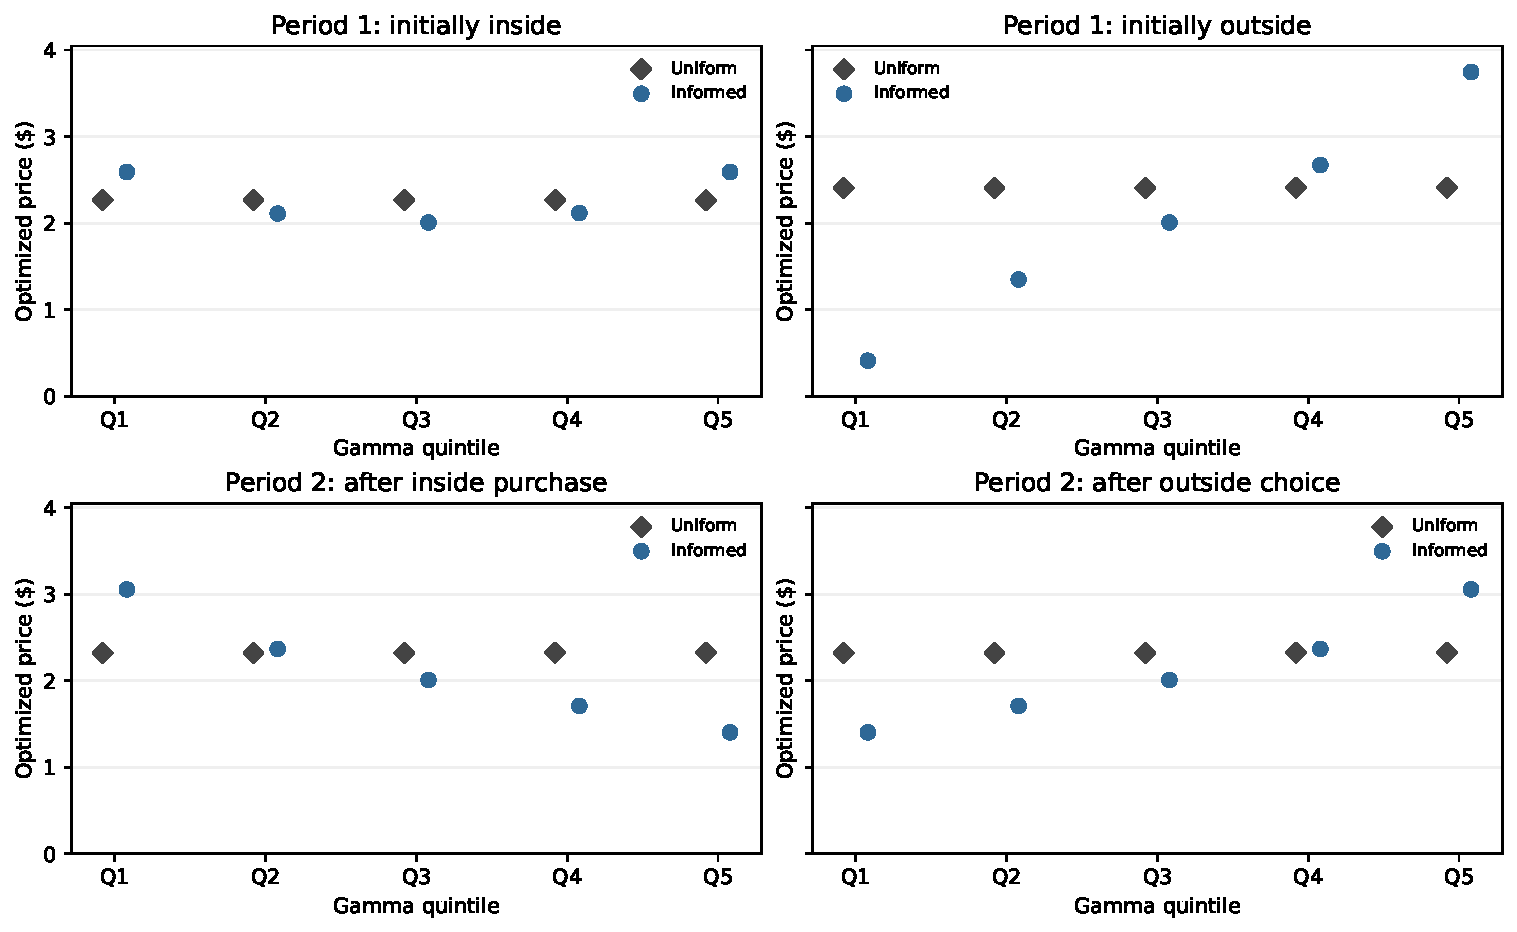
\includegraphics[width=9.5in,height=5.4in,keepaspectratio]{advisor_assets/theory_prices.pdf}
\end{center}
Each quintile has 20\% probability. Points are optimized offers at the indicated decision,
without averaging over future purchase histories. The informed firm knows the quintile, not exact gamma.
\newpage
\titleline{Theory benchmark: welfare and revenue}
\small
Percentage changes are Informed minus Uniform, divided by the absolute Uniform baseline.
CS uses zero outside utility; TW is CS plus revenue.
\begin{center}
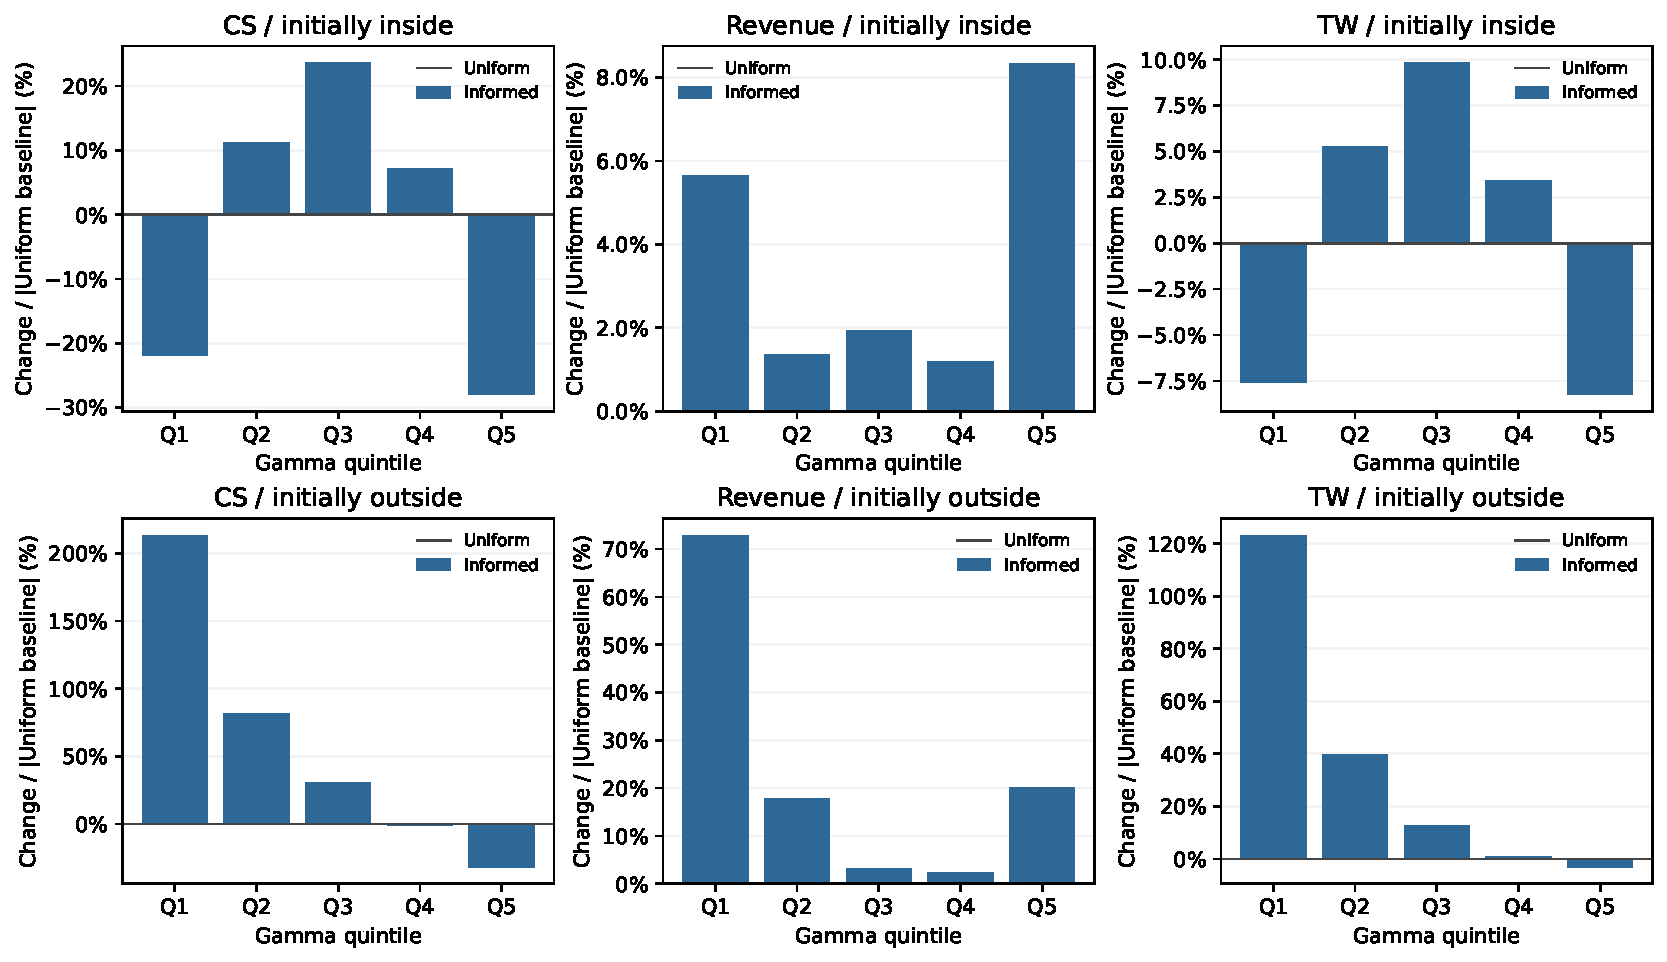
\includegraphics[width=9.8in,height=5.95in,keepaspectratio]{zero_outside/assets/theory_welfare.pdf}
\end{center}
\newpage
\titleline{Plain prices: trimmed, flavor switching specification}
\small
Gamma is trimmed at the 5th and 95th percentiles, with the retained distribution renormalized.
All offered prices are constrained to be nonnegative.
\begin{center}
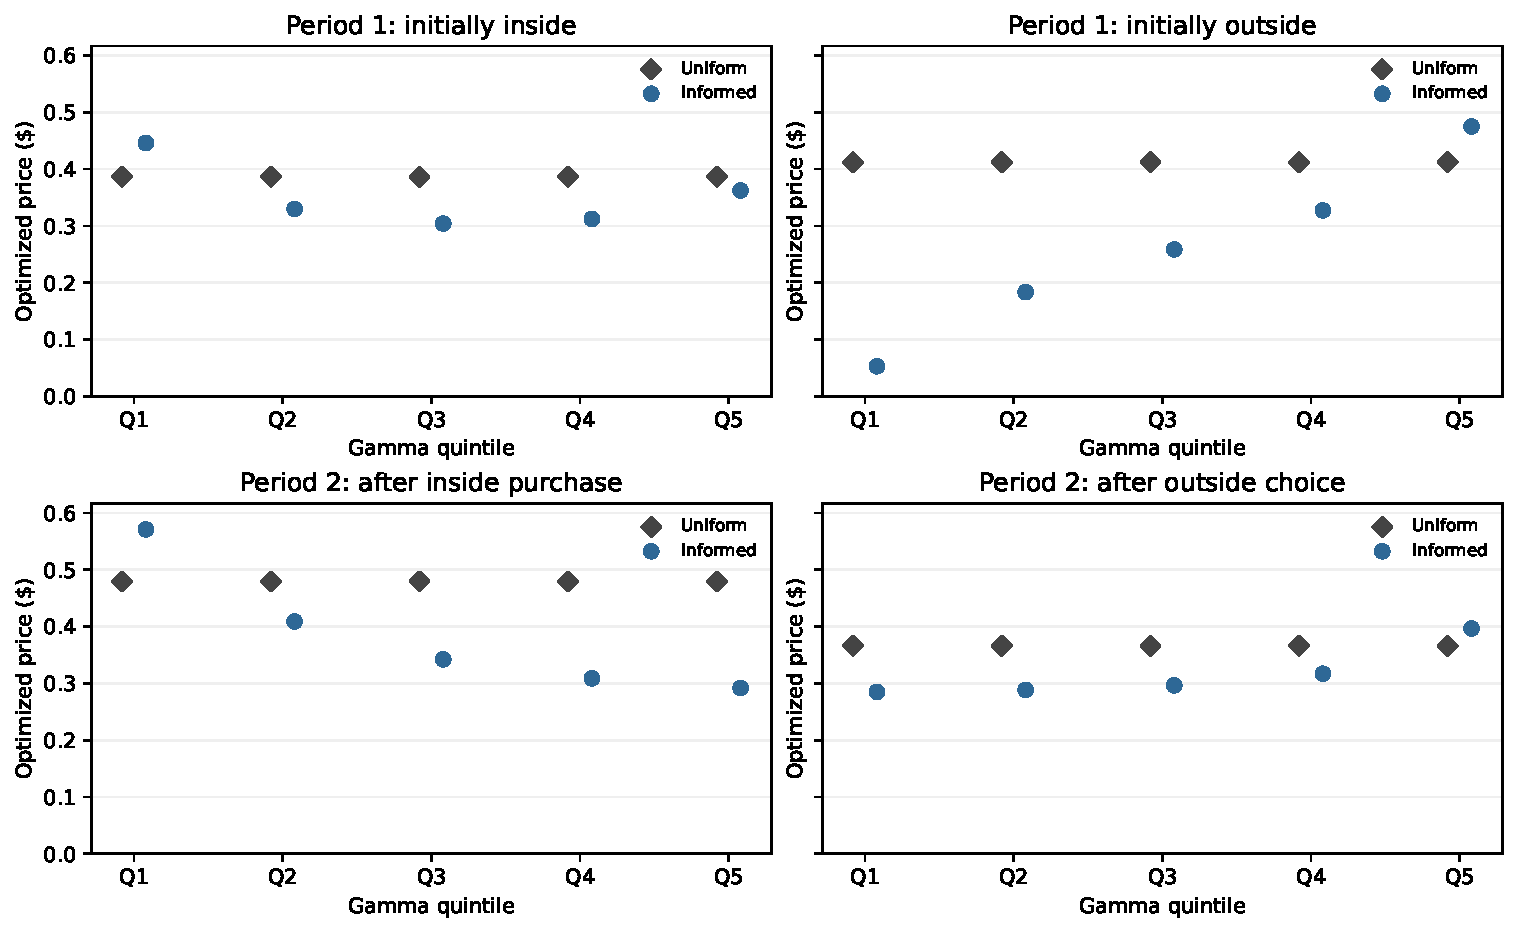
\includegraphics[width=9.5in,height=5.35in,keepaspectratio]{advisor_assets/plain_prices.pdf}
\end{center}
Inside means plain yogurt; outside means no plain yogurt (berry, other yogurt, or no yogurt).
Q1--Q5 each contain 20\% of the retained distribution (18\% of original mass).
\newpage
\titleline{Plain welfare: trimmed, flavor switching specification}
\small
Percentage changes are Informed minus Uniform, divided by the absolute Uniform baseline.
CS uses zero outside utility; TW is CS plus revenue.
\begin{center}
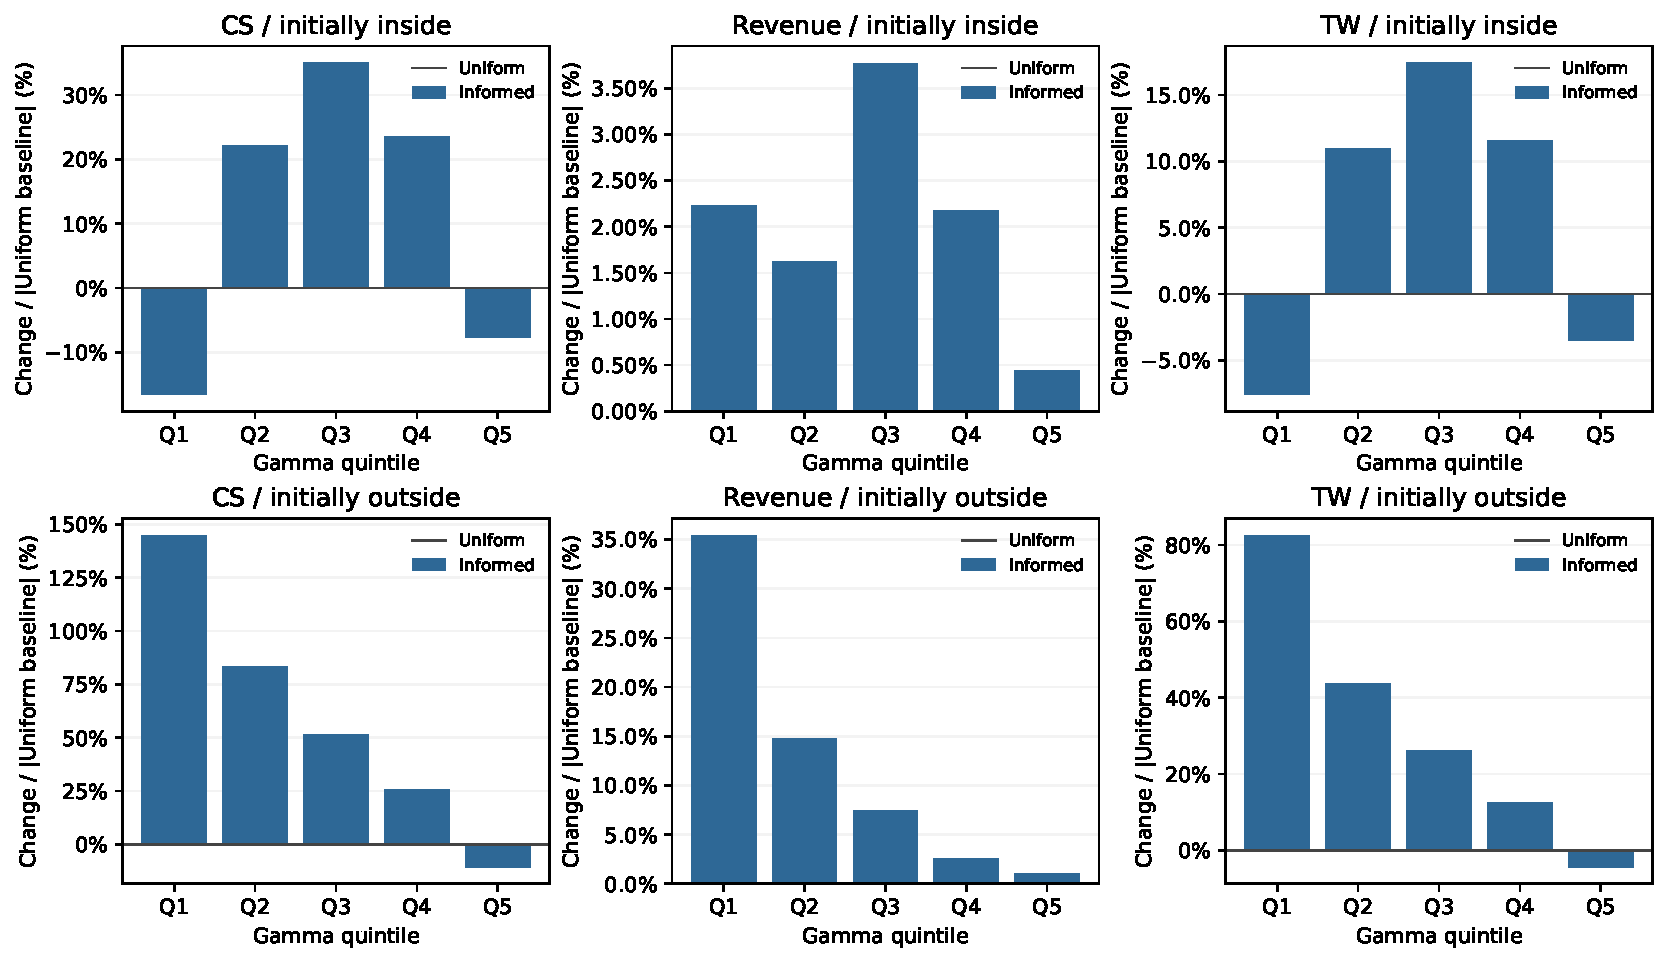
\includegraphics[width=9.8in,height=5.95in,keepaspectratio]{zero_outside/assets/plain_welfare.pdf}
\end{center}
\newpage
\titleline{Welfare outliers: dollar levels and percentage changes}
\small
Trimmed, flavor switching specification. Values are expected dollars per consumer
over the two modeled shopping weeks, conditional on the stated initial state and quintile.
CS uses zero outside utility; TW is CS plus revenue at zero cost.
\vspace{10pt}
\begin{center}
\renewcommand{\arraystretch}{1.4}
\begin{tabular}{lllrrrr}
\toprule
Initial state & Quintile & Metric & Uniform (\$) & Informed (\$) & Change (\$) & Change (\%)\\
\midrule
Outside & Q1 & CS & 0.00248 & 0.00608 & +0.00360 & +145.0\% \\
Outside & Q1 & TW & 0.00576 & 0.01052 & +0.00476 & +82.6\% \\
\addlinespace
Inside & Q1 & CS & 0.44577 & 0.37188 & -0.07389 & -16.6\% \\
Inside & Q1 & TW & 0.85526 & 0.79049 & -0.06477 & -7.6\% \\
\addlinespace
Outside & Q5 & CS & 0.14482 & 0.12921 & -0.01561 & -10.8\% \\
Outside & Q5 & TW & 0.31435 & 0.30059 & -0.01376 & -4.4\% \\
\bottomrule
\end{tabular}
\end{center}

\newpage
\titleline{Symmetric switching: start with the choice, then take the difference}
\small
Let $j$ mean plain yogurt and $0$ mean not plain (berry, other yogurt, or no yogurt).
Let $h$ be the previous occasion's choice and $a_t$ the current choice.
The switching specification is
\[
u_t(a_t\mid h,\gamma)
=\mathbf1\{a_t=j\}(\beta+\alpha p_t)
+\gamma\mathbf1\{a_t\ne h\}+\varepsilon_{a_t t},\qquad \alpha<0.
\]
Gamma applies only when the choice changes. Negative gamma discourages switching;
positive gamma encourages it. Staying has no switching term.
\begin{center}
\renewcommand{\arraystretch}{1.4}
\begin{tabular}{lll}
\toprule
Previous choice & Choose plain: $V_j$ & Choose outside: $V_0$\\
\midrule
Plain & $\beta+\alpha p$ & $\gamma$\\
Outside & $\beta+\alpha p+\gamma$ & $0$\\
\bottomrule
\end{tabular}
\end{center}
With independent Type-I extreme-value choice shocks, the plain purchase probability is
\[
q_h(p,\gamma)=\frac{e^{v_h(p,\gamma)}}{1+e^{v_h(p,\gamma)}},\qquad
v_h=V_j-V_0=
\begin{cases}
\beta+\alpha p-\gamma,&h=j,\\
\beta+\alpha p+\gamma,&h=0.
\end{cases}
\]
The minus sign after a plain purchase comes from subtracting the utility of leaving.
It is not a switching term on repeating plain. Thus low gamma makes staying more
attractive and entering less attractive. With $a=-\alpha>0$, the prices at which the
two deterministic utilities are equal are
\[
WTP_j(\gamma)=\frac{\beta-\gamma}{a},\qquad
WTP_0(\gamma)=\frac{\beta+\gamma}{a}.
\]
These are willingness to pay relative to the outside option; choice shocks still allow either choice.
\newpage
\titleline{What the zero-outside welfare measure reports}
\small
At a given history, subtracting $V_0$ from both alternatives gives the same purchase
probability. This packet reports the value of having plain available relative to
having only the outside option at that history:
\[
C_h^Z(p,\gamma)
=\frac{\log(e^{V_j}+e^{V_0})-V_0}{a}
=\frac{\log(1+e^{v_h(p,\gamma)})}{a}.
\]
For a policy $(p_1,p_{2j},p_{20})$, write $q_1=q_{h_0}(p_1,\gamma)$.
Period 2 follows the period-1 choice: plain with probability $q_1$, outside with probability $1-q_1$.
\begin{align*}
CS^Z(\gamma,h_0)
&=C_{h_0}^Z(p_1,\gamma)
+\delta\left[q_1C_j^Z(p_{2j},\gamma)+(1-q_1)C_0^Z(p_{20},\gamma)\right],\\
R(\gamma,h_0)
&=p_1q_1+\delta\left[q_1p_{2j}q_j(p_{2j},\gamma)
+(1-q_1)p_{20}q_0(p_{20},\gamma)\right],\\
TW^Z(\gamma,h_0)&=CS^Z(\gamma,h_0)+R(\gamma,h_0).
\end{align*}
\textbf{Distinction from welfare in the original switching utilities.}
Keeping the original utility levels instead gives
\[
C_h^O=C_h^Z+\frac{\gamma}{a}\mathbf1\{h=j\},\qquad
CS^O-CS^Z=\frac{\gamma}{a}\left[\mathbf1\{h_0=j\}+\delta q_1\right].
\]
Therefore, for Informed minus Uniform at the same initial history and gamma,
\[
\Delta CS^O-\Delta CS^Z=\frac{\delta\gamma}{a}(q_1^I-q_1^U).
\]
Subtracting outside utility is harmless for choice probabilities. It need not be
harmless for two-period welfare comparisons, because prices change the probability
of each future history. The figures here use the history-relative measure $CS^Z$
and its associated $TW^Z$, rather than the original utility-level measure.
The common extreme-value shock constant is omitted throughout.
\newpage
\titleline{Pricing, aggregation and maintained assumptions}
\small
Consumers choose myopically; gamma is persistent. Uniform knows history and the
population distribution $G$, but not quintile. Informed also knows quintile and uses
its conditional distribution. There is no learning: each information set keeps its
same distribution after either choice. The population distribution is assumed identical
across initial histories. Prices are nonnegative, marginal cost is zero and $\delta=1$.

For the relevant fixed distribution $F$, terminal offers solve
\[
p_{2h}\in\arg\max_{p\geq0}\int p q_h(p,\gamma)\,dF(\gamma),\qquad h\in\{j,0\}.
\]
Define $r_h(\gamma)=p_{2h}q_h(p_{2h},\gamma)$. The first-period offer solves
\[
p_1(h_0)\in\arg\max_{p\geq0}\int\left[
 p q_{h_0}(p,\gamma)+\delta\left\{
 q_{h_0}(p,\gamma)r_j(\gamma)
 +(1-q_{h_0}(p,\gamma))r_0(\gamma)\right\}\right]dF(\gamma).
\]
Purchase probabilities and future revenue remain paired for the same persistent type
inside the integral. At an interior optimum the price derivative is zero; at zero price
it is nonpositive. Changing the welfare baseline does not change this revenue problem:
this packet retains the symmetric-switching prices and revenue.

Each quintile outcome is the mean over its conditional distribution $F_k$:
\[
\overline M_k^r(h_0)=\int M^r(\gamma,h_0)\,dF_k(\gamma),\qquad
\text{percentage change}=100\frac{\overline M_k^I-\overline M_k^U}{|\overline M_k^U|}.
\]
A zero baseline is undefined. The dollar table reports expected two-period dollars
per consumer, conditional on initial history and quintile.

\textbf{Applied calibration.}
Trimmed, flavor switching specification: $\beta_{plain}=-1.285109$, $\alpha=-3.530427$;
original gamma mean $-0.838193$, SD $2.099165$. Retain and renormalize the 5th--95th
percentile interval. Each quintile contains 20\% of retained probability. Alpha and beta
are fixed; no demand model is refitted. These are conditional-history calculations,
not a new run on household records.

\textbf{Theory calibration.}
$\beta=2$, $\alpha=-1$, $\gamma\sim N(0,1.25^2)$ without trimming.
The same information structure, symmetric switching, price constraint and welfare measure apply.
\end{document}
